\chapter{Machine-learning algorithms for intrusion detection systems}
\label{cha:2}
The main task in statistical learning is to avoid any \emph{overfitting}: any useless addition of complexity may allow the regression to capture the variance of the specific data-set on which it is trained on top of the underlying relation is it supposed to capture. The regression would then reproduce the training set itself instead of generalising it. I therefore would like to cite John von Neumann
\begin{displayquote}
\emph{With four parameters I can fit an elephant, and with five I can make him wiggle his trunk.}
\end{displayquote}

In other words, one parameter is sufficient to add a lot of complexity to the model and increase a lot the risk of overfitting. The general rule of thumb is thus to always reduce as much as possible the complexity of the model and always stick to the lowest one able to reproduce the general scheme of the data. This principle is also known as \emph{Occam's razor}.

\section{Intrusion Detection Systems}
\emph{Intrusion detection systems} (IDS) are a brick in the existing defence algorithms arsenal wall of information security. More specifically, it includes a series of mechanisms that monitor network nodes and detect intrusions, i.e. malicious activity or policy violations. An IDS usually analyzes the incoming packets and tries to detect the suspect ones. In most cases, IDS are defined to be the sole surveillance application and do not comprise the control application: how the suspect packets are treated after a notification is not considered as being part of the IDS, the latter only focuses on the monitoring, analysis and notification \cite{Mukherjee1994NetworkDetection}. Classically, the reports are made to an administrator or another competent entity, as \emph{security information and event management} (SIEM) \cite{Bhatt2014TheSystems}, which are then in charge of the control application. 

IDS should not be confused with \emph{firewalls}, but merely be seen as a complement of it. The only role of firewalls is to ensure that communication policies are followed carefully. A first difference is that firewalls have an upstream role whereas IDS are working downstream. In other words, firewalls are verifying that each packet is following carefully one of the pre-defined allowed communication protocols, before it enters the local network. An IDS analyzes the packets after they enter the local network to control if they show no abnormal behaviour. Another difference has already been mentioned: firewalls consider each packet separately whereas IDS can consider group of packets and thus look at a communication as a whole. In this sense, IDS are much more suited against \emph{denial of service} (DoS) attacks than classical firewalls. A last difference concerns the exact scope of the packet analysis. As firewalls only have to enforce communication policies, they only have to look at the packet header, whereas IDS are searching for abnormal behaviours and are thus looking at the packets on the whole. To summarize this all, let's consider a high security building: the firewall would be equivalent to the agents allowing or not each individual to enter the site by carefully inspecting their papers, whereas the IDS would be the security agents monitoring the cameras inside to building searching for abnormal behaviour.

IDS should also not be confused with \emph{anti-viruses} applications --- though the term \emph{anti-malware} would be more suited nowadays --- that refer to the application layer in charge of the detection and control of malicious code, or malware. The first difference concerns the scope of their analysis: anti-viruses are analyzing (executable) code on a system more specifically than packets on a network. The second difference is similar as before: anti-viruses analyze code before it is allowed to be executed by the system and IDS analyze packets that already entered the network.

However, all these taxonomy classifications are to be considered with some flexibility. As the attacks become more and more sophisticated, security entities are incorporating more, and more subtleties are extending the scope of their detection methods. As such, they integrate other types of methods classically defined by other entities.

\subsection{How IDS work}
As briefly stated before, IDS have three main components: monitoring, analysis and notification. 

The monitoring can be achieved in real time or at regular interval on different types of nodes, which define the type of IDS: network based IDS (NIDS), host based IDS (HIDS) and hybrid if they monitor on both. 

The analysis is the core part of the IDS and is again divided in three main components: the extraction of features, the pattern analysis and the final classification \cite{Winter2018}. This will be the part which will interest us in this thesis.

As written before, the notification is done to a controller, either an administrator or a SIEM. Classically, this takes place in the form of a series of logs which are later examined by the controller. In this sense, the speed is not the main focus of an IDS, but rather the correct identification of intrusions. However, one can also consider \emph{intrusion prevention systems} (IPS) which are working upstream. The literature sometimes considers these systems to be a specific class of IDS or to be a category on their own. However in opposition to IDS, IPS need to be fast and thus usually use signature-based detection. In this sense, IPS can be seen as an extension of firewalls as they also analyze the content of packets and not just the enforcing of protocols. Taking the IPS into account, one should still consider analysis speed in IDS.

The general structure of IDS is summarized at figure~\ref{img:ids-model}.

\begin{figure}[t]
    \centering
    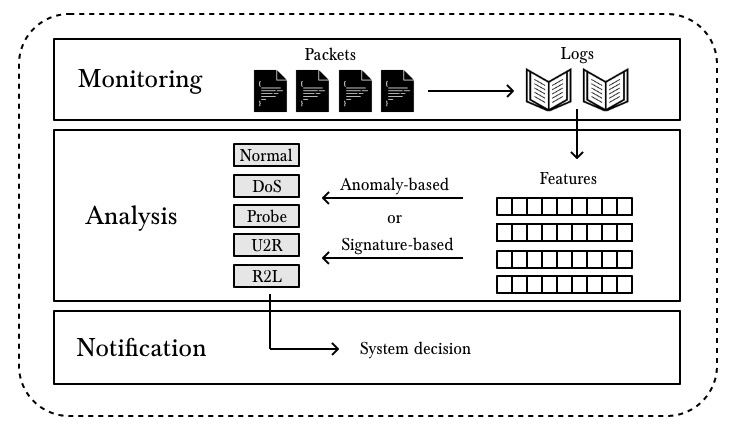
\includegraphics[width=.95\textwidth]{parts/chap-2/img-2/ids-model.jpg}
    \caption[Structure of an intrusion detection system]{General structure of an intrusion detection system. The different attack classes are based here on chapter~\ref{cha:4}.} 
    \label{img:ids-model}
\end{figure}

\subsection{Extraction of features}
Packets to be analyzed have a huge size and cannot be analyzed as such by the IDS. They typically incorporate huge redundancy and other non-necessary information such as padding. The idea of feature reduction is to reduce the packets to a limited number of features, representing as much non-redundant information as possible. Examples of features extracted consist of the connection length, the protocol used, the number of bytes transferred from the source to the destination and vice-versa.


\subsection{Pattern analysis}
The goal of the analysis of the IDS is to categorize the packets into different classes, typically a normal class and some different attack classes. As stated in the introduction, this can be done by two different manners based on a signature (\emph{signature-based}) and using some statistical rules (\emph{anomaly-based}). In this thesis, we will interest us to anomaly-based IDS, more specifically using classification machine-learning algorithms. The goal is that a user is able to classify its (query) on external trained machine-learning algorithm from one or more other parties, called the model owner(s). Furthermore, these algorithms have to be privacy-friendly in the sense that nor the query, nor the information resulting from the training should be revealed. This chapter aims at describing the two main machine-learning algorithms used without any consideration of the privacy-friendliness that will be covered in chapter~\ref{cha:3}.

\FloatBarrier
\section{Data reduction}


\subsection{Instance set size reduction}
Instance-based learning algorithms are often faced with the problem of deciding which instances to store for use during generalization. Storing too many instances can result in large memory requirements and slow execution speed, and can cause an oversensitivity to noise. \noteH{Input size so big as possible to reduce variance of the results}

In the practice, the data can be classified into two kind of classes, attack and no attack, or normal. In a practical intrusion detection system, most of the traffic is normal and sole a few proportion is attacking. We thus want to reduce the size of the normal data-set to make it of a similar size to the attack classes. Furthermore, the normal instances are very diversified and one may not just reduce the set randomly in the risk of missing relevant instances. One must thus find a more intelligent heuristic to decide which normal instances to keep.

How to decide which instances keep?
Keep only the ones near to the decision boundary. (+ explain what is a decision boundary). Way of keeping the sole normal instances near the decision boundary out of a way bigger set and thus build a more relevant training set of normal instances.

\subsubsection{$k$-means clustering}
The $k$-means clustering algorithm is a semi-supervised instance set reduction algorithm. This a specific case of clustering methods, that aim to divide the original data-set into smaller $k$ smaller clusters that should share some common properties. The challenge here is to find the most homogeneous possible clusters, which instances are similar enough --- referred to as the minimisation of \emph{intra-class inertia} ---, but not too many so that the clusters are well differentiated -- also referred to as the maximiastion of \emph{inter-class intertia}. After this being achieved, one can thus reduce each cluster far from the decision boundary to an archetype instance of this cluster and keep the clusters near the decision boundary. The algorithm is semi-supervised as the clustering in itself is only based on the features set, but is only applied on the data-points that are classified as normal, which of course depends on the target space.

To determine the different clusters, the $k$-means algorithm tries to minimize the distance between the instances in each cluster $\mathcal{S}_i$. The number clusters is fixed to $k$, which an hyper-parameter of the model set by the user. Computing the distance between each of the points would require a quadratic at each evaluation of cluster. To keep the complexity linear, the distances are not computed between each of the instances, but between each of the instances and the mean of these instances $\mu_i = \left( \sum_{x_j \in \mathcal{S}_i} x_j\right)/\vert \mathcal{S}_i \vert$ where $\vert \mathcal{S}_i \vert$ is the number of instances in the cluster.
\begin{equation}
    \underset{\mathcal{S}}{\mathrm{arg}\,\mathrm{min}} \sum_{i=1}^k \sum_{x_i \in \mathcal{S}_i} \norm{x_j-\mu_i}^2
\end{equation}
Defining the optimal clusters would at least be exponentially complex in function of the number of total instances as each cluster combination would have to be tested. Therefore, the $k$-means algorithm starts with assigning the starting clusters to initial data-points, chosen at random in our case. It then goes through the whole data-set and assigns each point to the cluster with the nearest mean $\mu_i$. The means are then updated and the process starts again. This is given at algorithm~\ref{alg:k-means}. Although doesn't guarantees any optimality nor polynomial computational time, it is considered very effective in the practice \cite{Arthur2006Worst-caseMethod}.

\begin{center}
\begin{algorithm}[H]
 \KwData{Feature data-set $\mathcal{F} = \left\{x_i\right\}_{i=1 \ldots n}$ and number of cluster sets $k$}
 \KwResult{$k$ clusters $\mathcal{S}_i = \left\{x_i\right\}_{i=1 \ldots m_i}$}
\DontPrintSemicolon

\lForEach{i = 1\ldots k}{
$\mu_i \leftarrow$ random $x_j$
}
\Repeat{$\mathrm{convergence}$}{
\ForEach{$x_j \in \mathcal{F}$}{
\lForEach{$i = 1\ldots k$}{$d_{i} \leftarrow \norm{x_j-\mu_i}$ \;}
$l \leftarrow \mathrm{arg}\,\mathrm{min} d_i$ \;
assign $x_j$ to $\mathcal{S}_l$ \;
}
\ForEach{$i = 1\ldots k$}{
$\mu_i \leftarrow \mu_i = \frac{1}{\vert \mathcal{S}_i \vert}\left( \sum_{x_j \in \mathcal{S}_i} x_j\right)$
}
}
\Return{$\mathcal{S}_{1 \ldots k}$}
\caption{The $k$-means algorithm. The convergence criterion typically is no more evolution in the means or the composition of the clusters, which is almost always equivalent in the practice.}
\label{alg:k-means}
\end{algorithm}
\end{center}

Once the clusters are determined, we can remove the normal data instances of the farthest from the decision boundary and replace the whole cluster by its mean $\mu_i$. In this way, we reduce the number of points far from the decision boundary and keep all the ones near the decision boundary. The number of set to be reduced $p<k$ is also an hyper-parameter set by the user. A way to determine which one are the farthest is just to compute the distance between the mean of each cluster and the mean of the attack instances defined in the same way.

\subsection{Feature size reduction}
+ explain why reduce the feature size. Complexity gain and better suited for distance calculation. Avoid curse of dimensionality. Avoid participation of non-relevant features in the training of the classification algorithm.

\subsubsection{Principal components analysis}
A linear Principal Components Analysis dimensionality reduction consists in a spectral analysis of the covariance matrix $\mathbf{\hat{\Sigma}}$ \noteH{(+ give forula for covariance matrix)} which can diagonalized with nonnegative eigenvalues $\lambda_i$ as it is semi-positive definite
\begin{equation}
\hat{\Sigma}x = \lambda_ix
\end{equation}
The $M$ greatest eigenvalues are then kept and the data transformed accordingly:
\begin{equation}
z_i = x_i^Tx
\end{equation}
Here is an attempt of an intuitive understanding of the process. Each input variable of the original input vector is independent, but some have strong underlying relations between them, measured by their covariance matrix. By diagonalizing it, there result $n_f$ new variables without any linear underlying relation. In a certain way, the eigenvectors $x_j$ represent these relations and their respective eigenvalues $\lambda_j$ their contribution, thus their importance. We can then afford to drop the non-important ones.

In our case, each feature is first being normalized, i.e. zero mean and unit variance. In other words, the covariance matrix has an unit diagonal and with a feature dimension of $n_f$, we have $tr(\hat{\mathbf{\Sigma}})=n_f$ which corresponds in a certain way to the total variance of the whole feature space. Quite logically, the latter is invariant to any linear transformation as the trace is an invariant to any linear transformation. The main idea behind linear PCA analysis reduction is thus to keep the richness of the data a maximum, thus its total variance, and reducing its dimension a maximum by dropping its smallest contributors. A good measure for the relative importance of each eigenvector, or underlying linear relation, is its fraction or variance contribution given by
\begin{equation}
f_j = \lambda_j/\Sigma_{\forall j}\lambda_j = \lambda_j/\tr\left(\hat{\mathbf{\Sigma}}\right)
\end{equation}

One can then choose the input values it decides to keep in descending order of the respective fractions $f_j$.

\subsubsection{Kernel principal components analysis and Mercer's trick}
The main problem of PCA is that it limits to linear relations between the feature elements. However, feature relations, especially in high dimension spaces require non-linear relations. Therefore, it would be interesting to map the instances into a space of higher dimension $\phi(x)$.

Therefore, we may now compute the covariance matrix in the mapped space $\phi\left( \mathcal{F} \right)$ of the feature space $\mathcal{F}$
\begin{equation}
    \hat{\Sigma}_{\phi} = \frac{1}{n_f} \sum_{x_i,x_j \in \mathcal{F}} \left( \phi(x_i) - \mathrm{mean} \right) \cdot \left( \phi(x_j) - \mathrm{mean} \right)
\end{equation}

Fortunately, there exists a method to compute this easily. Mercer's trick \cite{Minh2006MercersSmoothing}, also known as \emph{the kernel trick} can be used when an algorithm is based on the sole scalar product between feature vectors instances. It can then be replaced by a \emph{kernel matrix} representing the scalar product of the transformations.
\begin{equation}
    K_{ij} = K(x_i,x_j) = \phi(x_i) \cdot \phi(x_j)
\end{equation}

To compute the covariance matrix, we first have to centralize the data, which can be easily done with simple matrices multiplication
\begin{eqnarray}
    K_{ij}'&=& K_{ij} - \frac{2}{n_f} \sum_k^{n_f}\left( K_{ik}+K_{jk} \right) + \frac{1}{n_f^2} \sum_{l,m,n,o}^{n_f}K_{lm}K_{no} \\
    K' &=& K - 1_{n_f}K - K1_{n_f}+ 1_{n_f}K1_{n_f}
\end{eqnarray}
where $1_{n_f}$ represents matrices of the size $\left( n_f , n_f \right)$ where all elements are equal to $1/n_f$.

We can now perform a diagonalization on this new covariance matrix of the transformed data-points and perform the classification on them. This method is called \emph{kernel principal components analysis} (KPCA). 

A very interesting property of the kernel matrix is there is no need for computing the explicit transformation of each data-point as we are only interested in their scalar product. Indeed, they are never used on their own, but always in the kernel matrix. As such, one may directly compute the direct matrix. This is even more interesting as the scalar product of most of the transformations are mapped into an infinite dimension feature space and the scalar product can only theoretically be computed in Hilbert sace. Different kernel functions are possible, that represent the scalar product of different transformations. These kernel functions rely more often on one or more hyper-parameter that has to be trained. The most common choices are
\begin{itemize}
    \item \textbf{Linear kernel function:} this corresponds to computing directly the scalar product onto the identity transformation $\phi(x_i)=x_i$ and is thus equivalent to a linear PCA analysis.
    \begin{equation}
        K(x_i,x_j) = x_i \cdot x_j
    \end{equation}
    \item \textbf{Radial basis function kernel function (RBF):} this kernel function has one hyper-parameter. At a scale factor excepted \noteH{(à une constante près ?)}, this corresponds to the probability of the second instance given the first one with standard deviation $\sigma$. An interesting property of this kernel function is its ability to measure similarity as it converges to zero as the distance between both data-points increase and the point thus becoming more and more dissimilar. RBF are known to have excellent generalization capabilities.
    \begin{equation}
        K(x_i,x_j) = e^{\frac{-\norm{x_i-x_j}^2}{2\sigma^2}}
    \end{equation}
    \item \textbf{Polynomial kernel function:} this kernel function also has one hyper-parameter $d$. In the practice, $d=2$ is often chosen as higher order tend to overfit.
    \begin{equation}
        K(x_i,x_j) = (x_i \cdot x_j +1)^d
    \end{equation}
\end{itemize}

Due to their strong generalization power, RBF kernel generally perform better than other kernels, especially if no additional knowledge of the data is available or multiclass problems as the different classes often are often more diverse and require more generalization. In the case of intrusion detection systems, RBF kernel functions also tend to show better results \cite{Kuang2014ADetection}. Though, other kernels seem to show better results in some specific binary cases \cite{Elkhadir2016IntrusionMethods}. In our case and as we will work with multi-class classifiers, we will also opt for RBF kernel functions.

\subsubsection{Chi-square feature selection}
Up to new, the idea was to reduce the feature size by constructing new ones as transformations of the original feature vectors. However, one also choose to to select a number of features and just not care about the other ones. Another interesting property would be to be able to reduce the feature size in a supervised way, taking the machine learning algorithm into account. This can be tackled with $\chi^2$-feature reduction.

This feature selection method is based on the $\chi^2$ statistical hypothesis test that measures the dependence of two variables.





$\chi^2$-feature reduction test have successfully been applied to some machine learning algorithms for intrusion detection systems and seem to deliver better results than PCA or KPCA \cite{SumaiyaThaseen2017IntrusionSVM}.
\section{Support Vector Machines}
Support vector machines are a set of supervised machine learning algorithms than can be used either for classification or regression proposed by Vapnik in 1963 \cite{VapLer63}. The main idea originates with binary classification and consists of finding an optimal hyper-plane between the data-points separating both target classes.

\subsection{Linear support vector machines}
In its primal form, the support vector machine corresponds to the following minimization problem
\begin{equation}
    \begin{aligned}
& \underset{x}{\text{minimize}} 
& & \frac{1}{2}w^Tw + C \sum_{k=1}^N \xi_k \\
& \text{subject to}
& & y_i\left[ w \cdot x_i+b \right] \geq 1-\xi_i, \; i = 1, \ldots, N \\
& 
& & \xi_i \geq 0, \; i = 1, \ldots, N.
\end{aligned}
\end{equation}
This corresponds to finding a hyper-plane defined by the vector $w$ and intercept $b$ that separates all the data-points. The minimization of $w^Tw = \norm{w}^2$ corresponds to maximizing the margin between the hyper-plane and the nearest data-points. This is the criterion used to define an unique hyper-plane as an infinity that separates the data-points correctly may exist. Indeed, the nearest data-points $x$ are on the parallel hyper-plane $w^Tx-b= \pm 1$. The distance between the margin and the nearest point is thus $1/\norm{w}$. Maximizing it means minimizing $\norm{w}$ and due to the monotony of the norm $\norm{w}^2 = w^Tw$.

Of course, it can happen that no hyper-plane is able to classify all points correctly. Slack variables $\xi_k$ are therefore introduced. The trade-off between the best possible classification of the data-points (the contribution of the slack variables) and the maximizing of the margin is controlled by the box contraint parameter $C$.

New data-points (queries) are estimated as
\begin{equation}
    \mathtt{SVM}(x) = w \cdot x + b 
\end{equation}
The classification is given by the side of the hyper-plane on which the data-point resides which corresponds to taking the sign of this estimation.

In comparison to other machine learning algorithms like neural networks for example, the SVMs present the big advantage taking the form of a convex optimization problem. But their greatest strength in my opinion is the ability to use transformations for representing a non-linear separation. Therefore, we have to to work in the dual space, where the SVM optimization problem now reformulates
\begin{equation}
    \begin{aligned}
& \underset{\alpha_i}{\text{maximize}} 
& & \sum_{i=1}^N \alpha_i - \frac12 \sum_{i,j=1}^N \alpha_i \alpha_j y_i y_j (x_i \cdot x_j) \\
& \text{subject to}
& & 0 \leq \alpha_i \leq C \; i = 1, \ldots, N \\
& 
& & \sum_{i=1}^N\alpha_i y_i = 0.
\end{aligned}
\end{equation}
and the estimation of a new data-point now becomes
\begin{equation}
    \mathtt{SVM}(x) = \sum_{i=1}^N \alpha_i y_i (x_i \cdot x) + b
\end{equation}
The dual formulation gives its name to support vector machines. A new data-point is estimated based on the other vectors from the training size and their corresponding weights. The box constraint parameter here corresponds to the maximum weight of a support vector. In the case of privacy-friendliness, support vectors are very sensitive data as they directly represent instances from the original training data-set.

\subsection{Mercer's trick and non-linear support vector machines}
The main problem of support vector machines as described above is that they are limited to linear relations between the feature elements. However, feature relations, especially in high dimension spaces require non-linear relations. Therefore, it would be interesting to map the instances into a space of higher dimension $\phi(x)$.

The feature vectors are only appearing in the form of a scalar product, which allows us to use Mercer's trick. The idea is to replace the scalar products by a kernel function $K(x_i,x_j) = \phi(x_i) \cdot \phi(x_j)$. In most kernel functions, the feature vector is mapped into a space of infinite dimension. We thereby have to consider the scalar product in a Hilbert space to keep the mathematical sense of it: $\phi(x_i) \cdot \phi(x_j) = \langle \phi(x_i), \phi(x_j) \rangle_{\mathcal{H}}$.

We can define the kernel matrix as $K_{ij} = K(x_i,x_j)$. A very interesting property of the kernel matrix is there is no need for computing the explicit transformation of each data-point as we are only interested in their scalar product. Indeed, they are never used on their own, but always in the kernel matrix. As such, one may directly compute the direct matrix. This is even more interesting as the scalar product in Hilbert spaces are practically infeasible as such. Different kernel functions are possible, that represent the scalar product of different transformations. These kernel functions rely more often on one or more hyper-parameter that has to be trained. The most common choices are
\begin{itemize}
    \item \textbf{Linear kernel function:} this corresponds to computing directly the scalar product onto the identity transformation $\phi(x_i)=x_i$ and is thus equivalent to a linear PCA analysis.
    \begin{equation}
        K(x_i,x_j) = x_i \cdot x_j
    \end{equation}
    \item \textbf{Radial basis function kernel function (RBF):} this kernel function has one hyper-parameter. At a scale factor excepted, this corresponds to the probability of the second instance given the first one with standard deviation $\sigma$. An interesting property of this kernel function is its ability to measure similarity as it converges to zero as the distance between both data-points increase and the point thus becoming more and more dissimilar. RBF are known to have excellent generalization capabilities.
    \begin{equation}
        K(x_i,x_j) = e^{\frac{-\norm{x_i-x_j}^2}{2\sigma^2}}
    \end{equation}
    \item \textbf{Polynomial kernel function:} this kernel function also has one hyper-parameter $d$. In the practice, $d=2$ is often chosen as higher order tend to overfit.
    \begin{equation}
        K(x_i,x_j) = (x_i \cdot x_j +1)^d
    \end{equation}
\end{itemize}

Due to their strong generalization power, RBF kernel generally perform better than other kernels, especially if no additional knowledge of the data is available or multi-class problems as the different classes often are often more diverse and require more generalization. In the case of intrusion detection systems, RBF kernel functions also tend to show better results \cite{Kuang2014ADetection}. Though, other kernels seem to show better results in some specific binary cases \cite{Elkhadir2016IntrusionMethods}. In our case and as we will work with multi-class classifiers, we will also opt for RBF kernel functions.

The SVM dual formulation now becomes
\begin{equation}
    \begin{aligned}
& \underset{\alpha_i}{\text{maximize}} 
& & \sum_{i=1}^N \alpha_i - \frac12 \sum_{i,j=1}^N \alpha_i \alpha_j y_i y_j K(x_i, x_j) \\
& \text{subject to}
& & 0 \leq \alpha_i \leq C \; i = 1, \ldots, N \\
& 
& & \sum_{i=1}^N\alpha_i y_i = 0.
\end{aligned}
\end{equation}
with estimation
\begin{equation}
    \mathtt{SVM}(x) = \sum_{i=1}^N \alpha_i y_i K(x_i,x) + b
\end{equation}
However, there is also a downside: we are now facing an optimization problem in the dimension of the number of input instances and not of the dimension of the feature space anymore. This means that the number of support vector will drastically increase, which is a bad scenario for our privacy-friendly models. This is one of the investigated trade-offs.


\subsection{Multi-class SVMs}
The main problem of SVM for multi-class classification is that they are not natively suited for it. Indeed, SVM return a single number representing how far the tested data-point is from the hyper-plane. SVMs are by definition created for binary classification as the whole idea behind it is to separate the feature space into two parts. The kernel trick doesn't change anything to that as it only projects the data-point into a space of higher --- often unlimited --- dimension where a new hyper-plane is searched for, but still dividing this new higher dimension space into two parts.

Ideas for classifying SVMs into different classes could be for example to put the output number into bins. However, this is a very bad idea as it would in fact suggest that all the different classes are divided by parallel hyper-planes at a distances corresponding the the range of the bins, which range could also be trained (figure~\ref{mach:svm-model-gr-1}). It almost never occurs that one hyper-plane separates two classes perfectly, the fact that $n-1$ parallel hyper-planes separate the feature space according the the $n$ different classes is even less likely. This hypothesis is much too strong and must be discarded. We therefore have to use more than one SVM and combine them.

We will present here two different ways of combining SVMs that have both been tested in the case of intrusion detection systems \cite{Kuang2014ADetection}\cite{SumaiyaThaseen2017IntrusionSVM} and produce fairly similar results although they never have been compared using exactly the same model for the rest.

The first way and the most frequent one is to create $n$ different classifiers, each for a class, and to look at which one produces the best results. 
\begin{equation}
    \underset{k}{\mathrm{arg}\,\mathrm{min}}\left\{ \mathtt{SVM}_k (x_i)   \right\}_{1 \ldots n} 
\end{equation}
where $\mathtt{SVM}_k$ represents the SVM for each class $k$. Each classifier takes as binary input, +1 for the class and -1 for all the rest data-points  (figure~\ref{mach:svm-model-1}). A way of interpreting it is looking for which SVM the data-point lies the farthest from the hyper-plane, at its good size (i.e. positive). This can be graphically observed at figure~\ref{mach:svm-model-gr-2}. This is called the \emph{one-against-all} model.

\begin{figure}[ht!]
    \centering
    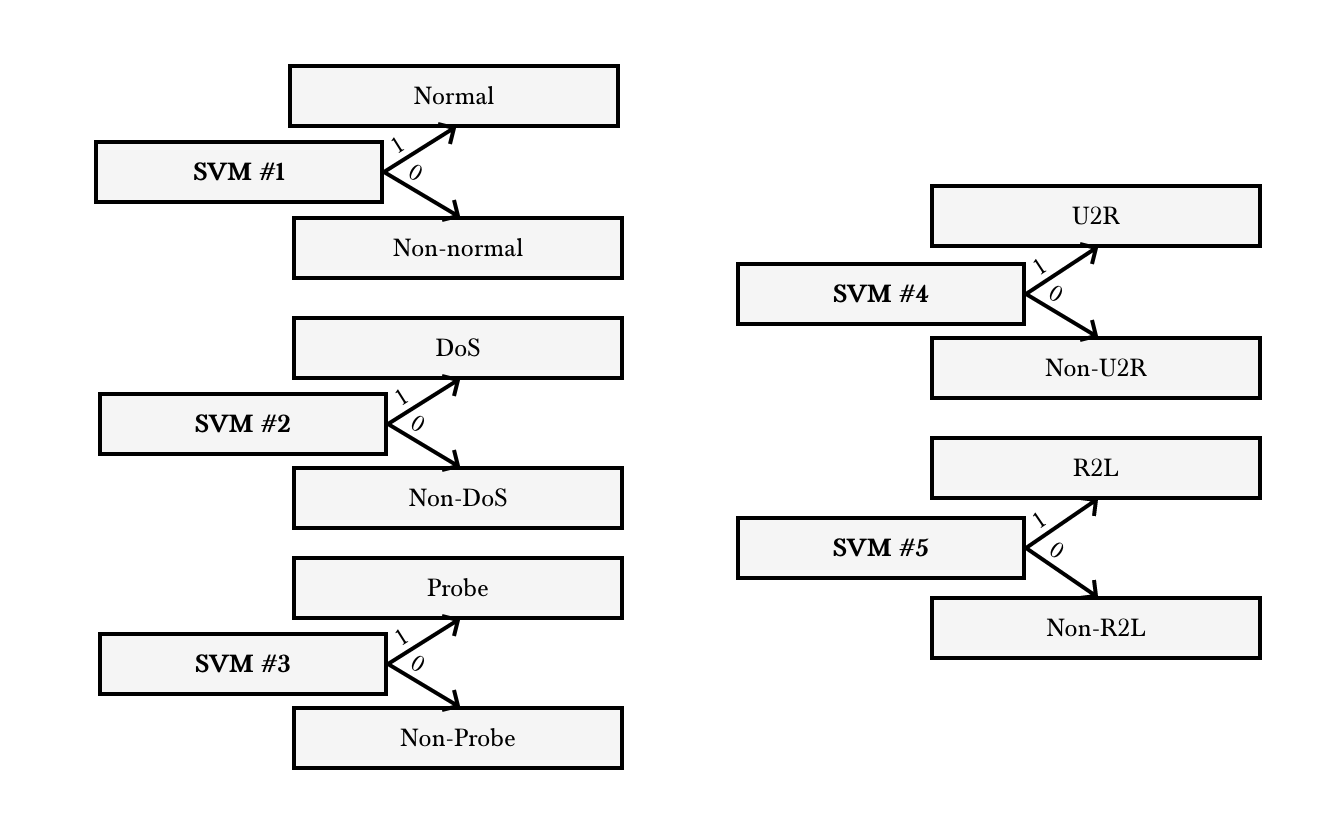
\includegraphics[width=.85\textwidth]{parts/chap-2/img-2/model-svm-1.png}
    \caption{One-against-all multi-class SVM model.} 
    \label{mach:svm-model-1}
\end{figure}

Another way of doing it is to work with successive SVMs as in figure~\ref{mach:svm-model-2} and is referred to as \emph{tree-based} models in this thesis. The first SVM is trained using one class as input versus all the others, as the first model. However the next classes are trained using one of the remaining classes versus the others remaining classes. The big advantage is that is only need $n-1$ different SVMs, which is one less compared to the previous model. Another advantage is that the last SVMs are trained one more specific data. However, the drawback is -- which is recurrent in series model --- that if one of the SVM isn't efficient, all the model is suffering. Graphically, this can be interpreted as first dividing the space with an hyper plane into two parts. One of the two parts is the subdivided into two new parts and so on (figure~\ref{mach:svm-model-gr-3}). Other tree structures are also to be considered, but this is not the scope of this thesis. We will limit ourselves to the consideration of these tree-structures in different orders. The goal of the machine-learning study of this thesis is to try to reduce the number of operations made by the evaluation of a query on the machine-learning algorithm. Computing 4 SVMs instead of 5 indeed decreases these number of computations. We thus want to investigate if this has an impact on the classification performance. A study on the comparison between the different tree-based models is a totally other subject which is not pursued here. We just limit ourselves to the different models found in the papers.

For the sake of completion, we also have to mention the existence of \emph{one-against-one} models where a binary classifier is trained for all combinations of two classes. The winning class it the one whose corresponding classifiers have the most positive outputs. However, this model needs $n_c(n_c-1)/2$ different classifiers where $n_c$ is the total number of classes, which is the opposite of the goal we are seeking.


\begin{figure}[ht!]
    \centering
    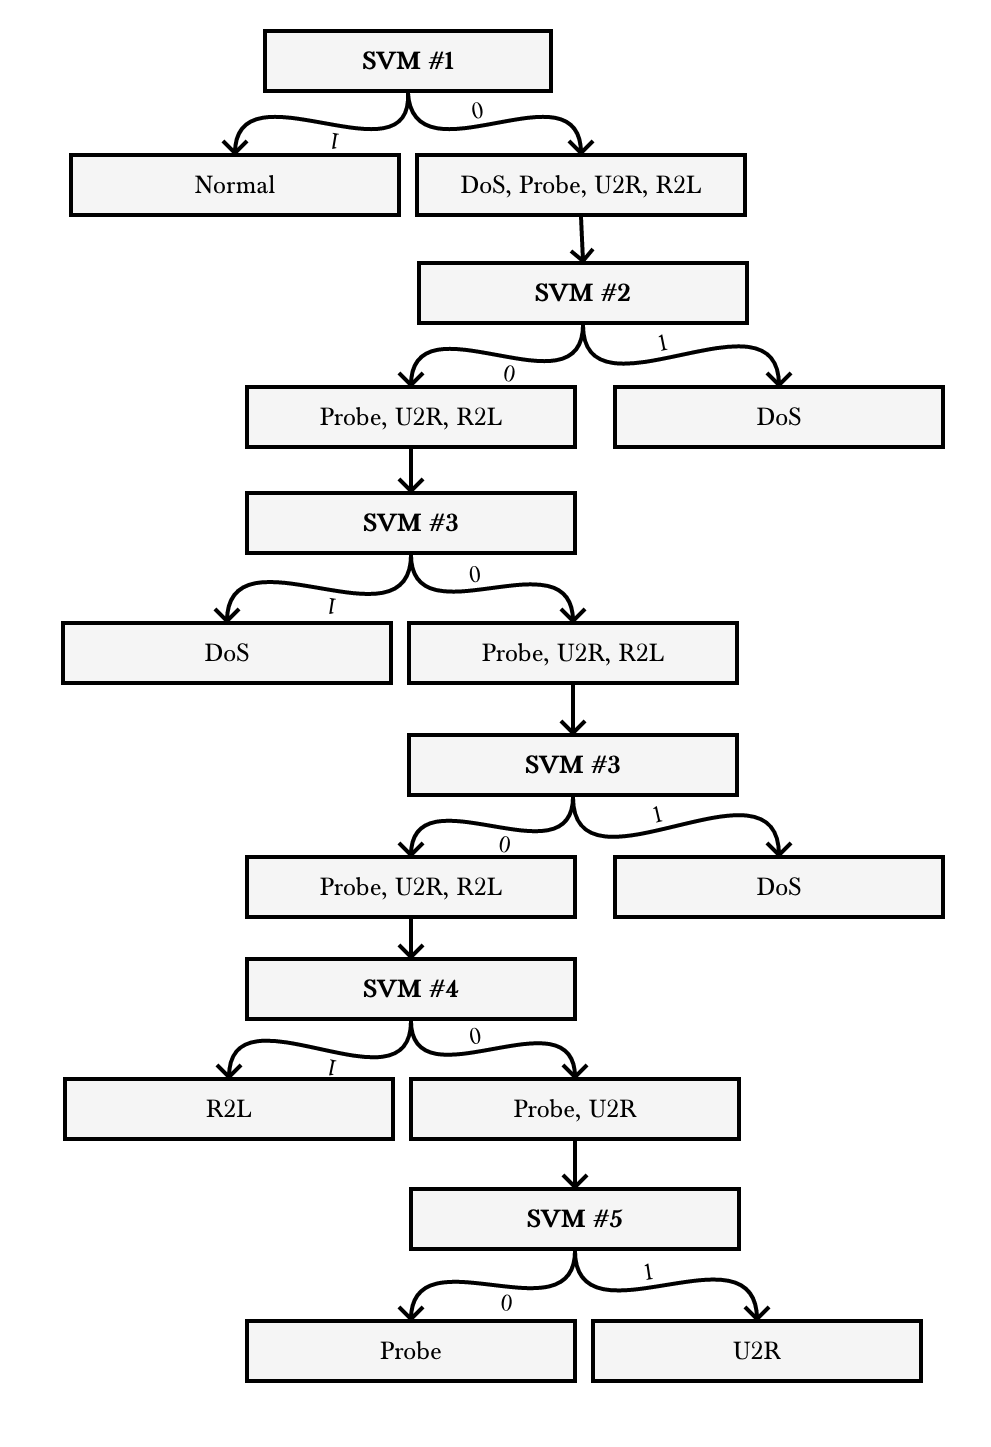
\includegraphics[width=.75\textwidth]{parts/chap-2/img-2/model-svm-2.png}
    \caption{Tree-based multi-class SVM model.} 
    \label{mach:svm-model-2}
\end{figure}

\begin{figure}
\begin{subfigure}[b]{0.32\textwidth}  
            \centering 
            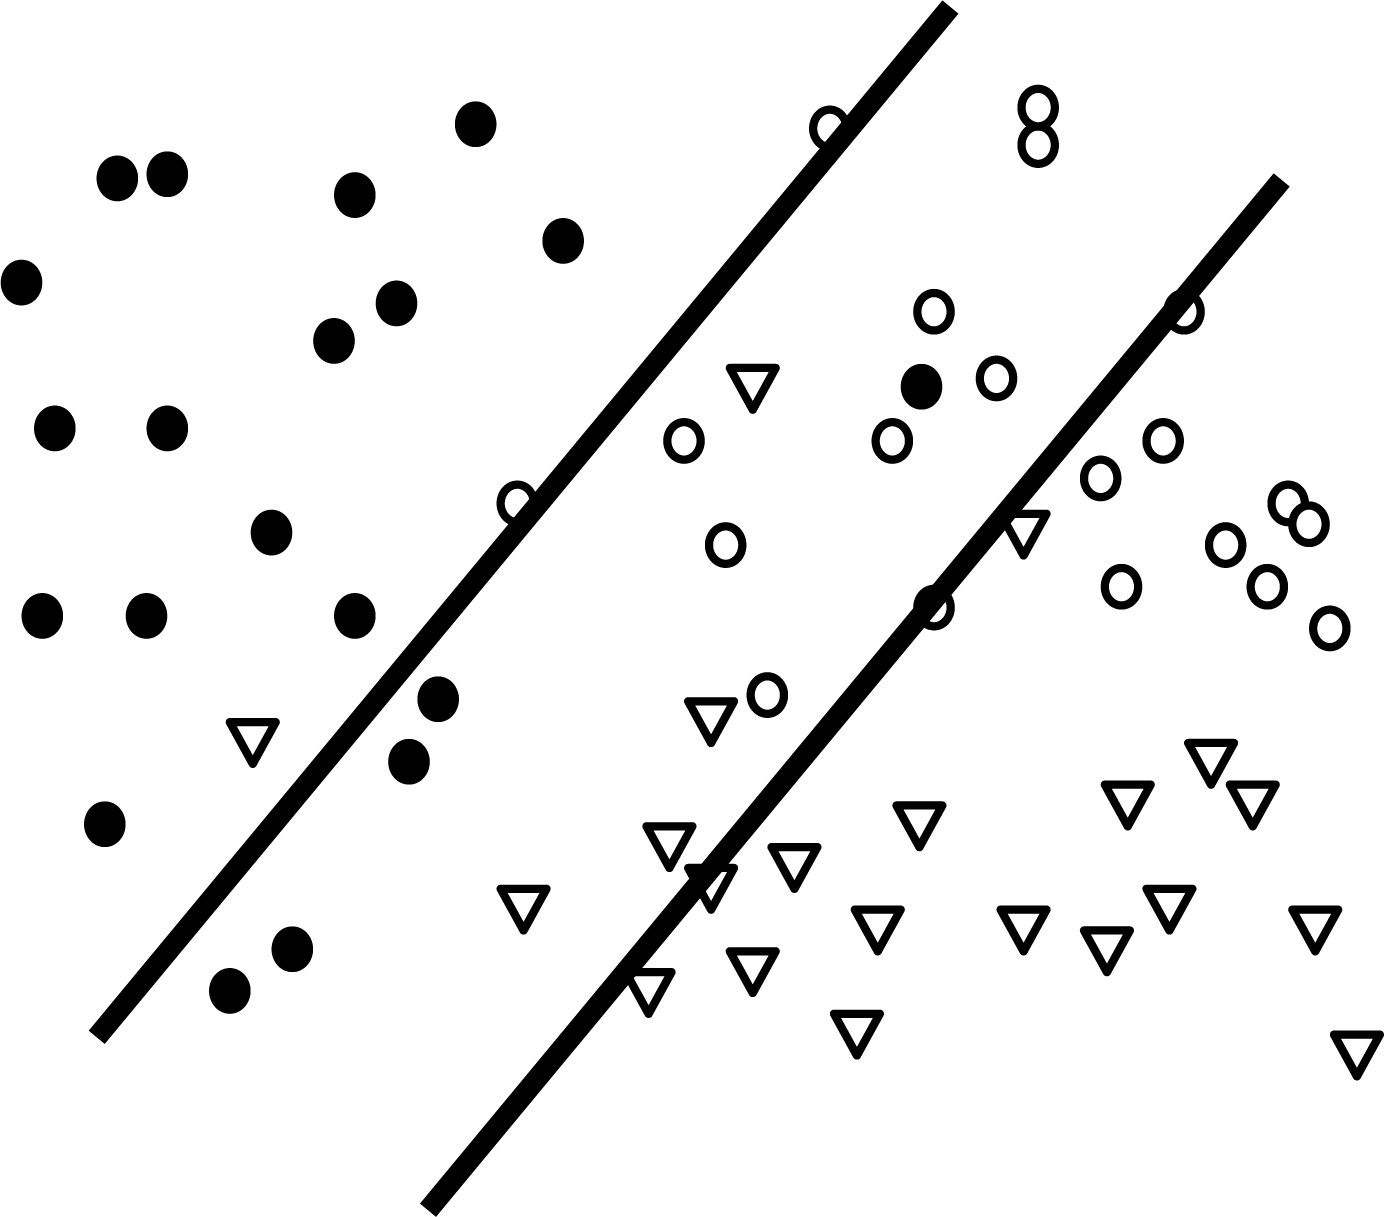
\includegraphics[width=.85\textwidth]{parts/chap-2/img-2/svm-par.png}
            \caption{Single SVM with bins.} 
            \label{mach:svm-model-gr-1}
        \end{subfigure}
        \hfill
        \begin{subfigure}[b]{0.32\textwidth}  
            \centering 
            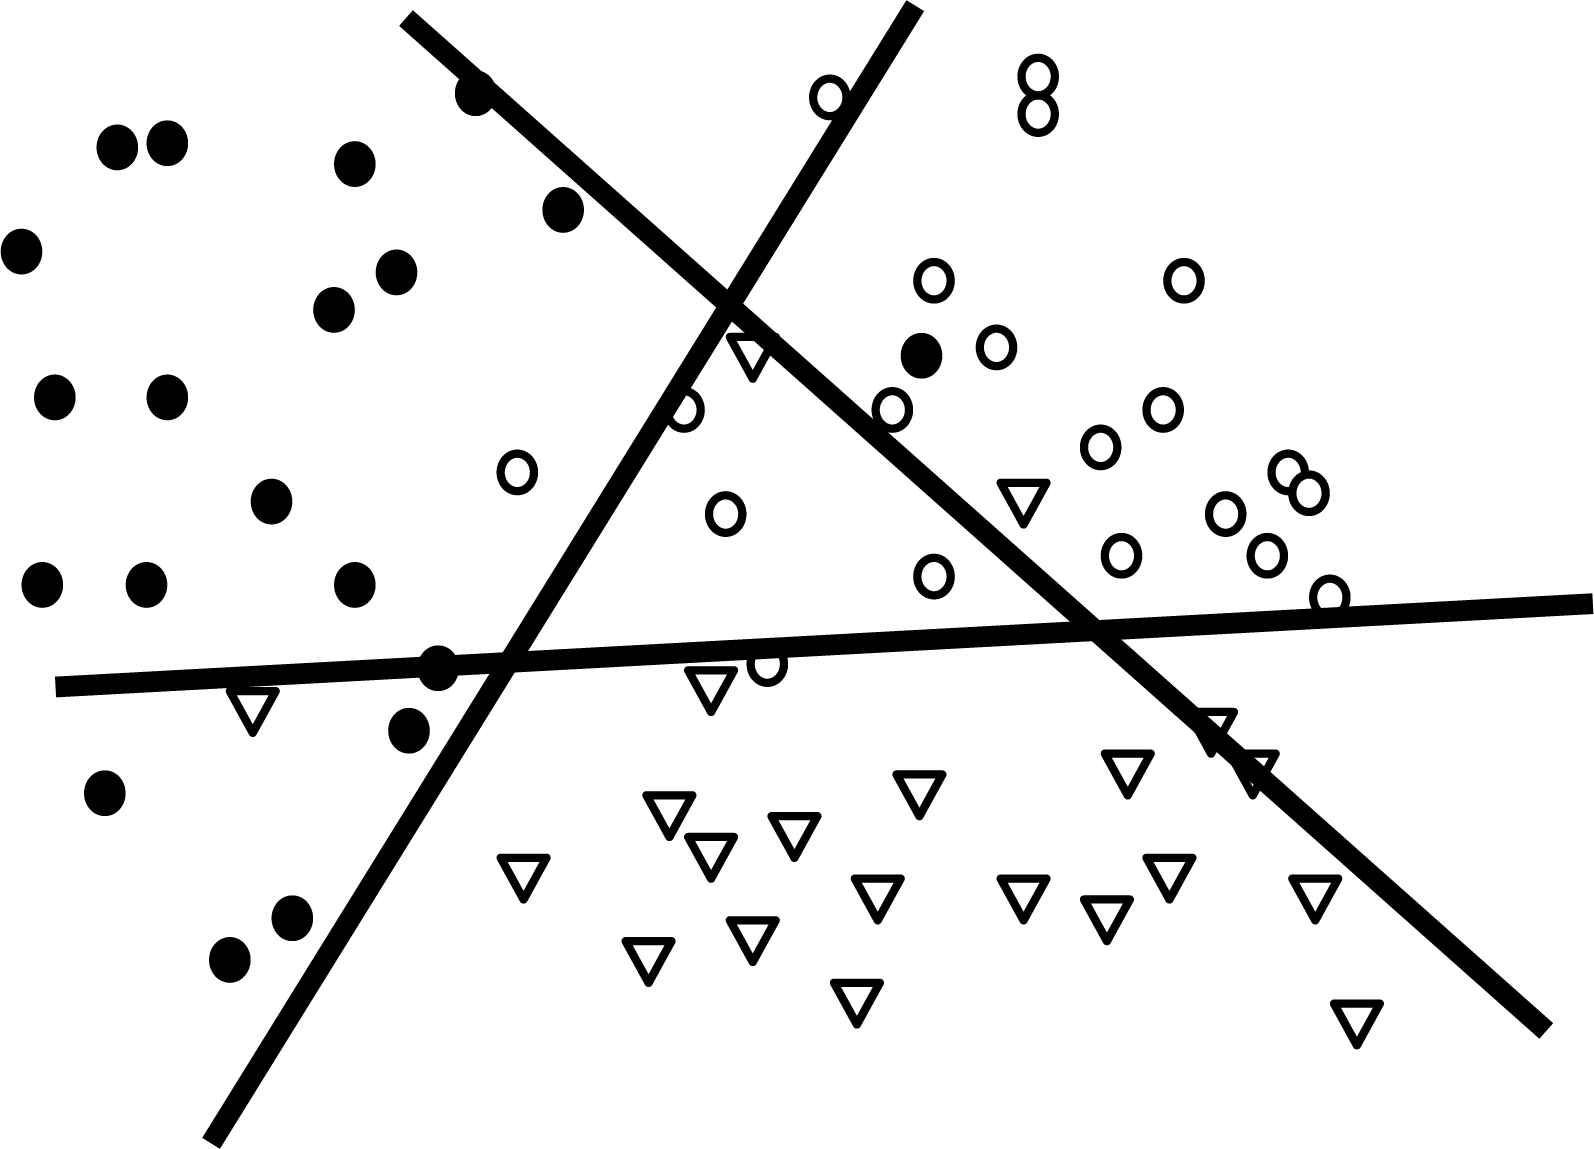
\includegraphics[width=.98\textwidth]{parts/chap-2/img-2/svm-multi.png}
            \caption{$n$ SVMs in a one-against-all model.} 
            \label{mach:svm-model-gr-2}
        \end{subfigure}
        \hfill
        \begin{subfigure}[b]{0.32\textwidth}   
            \centering 
            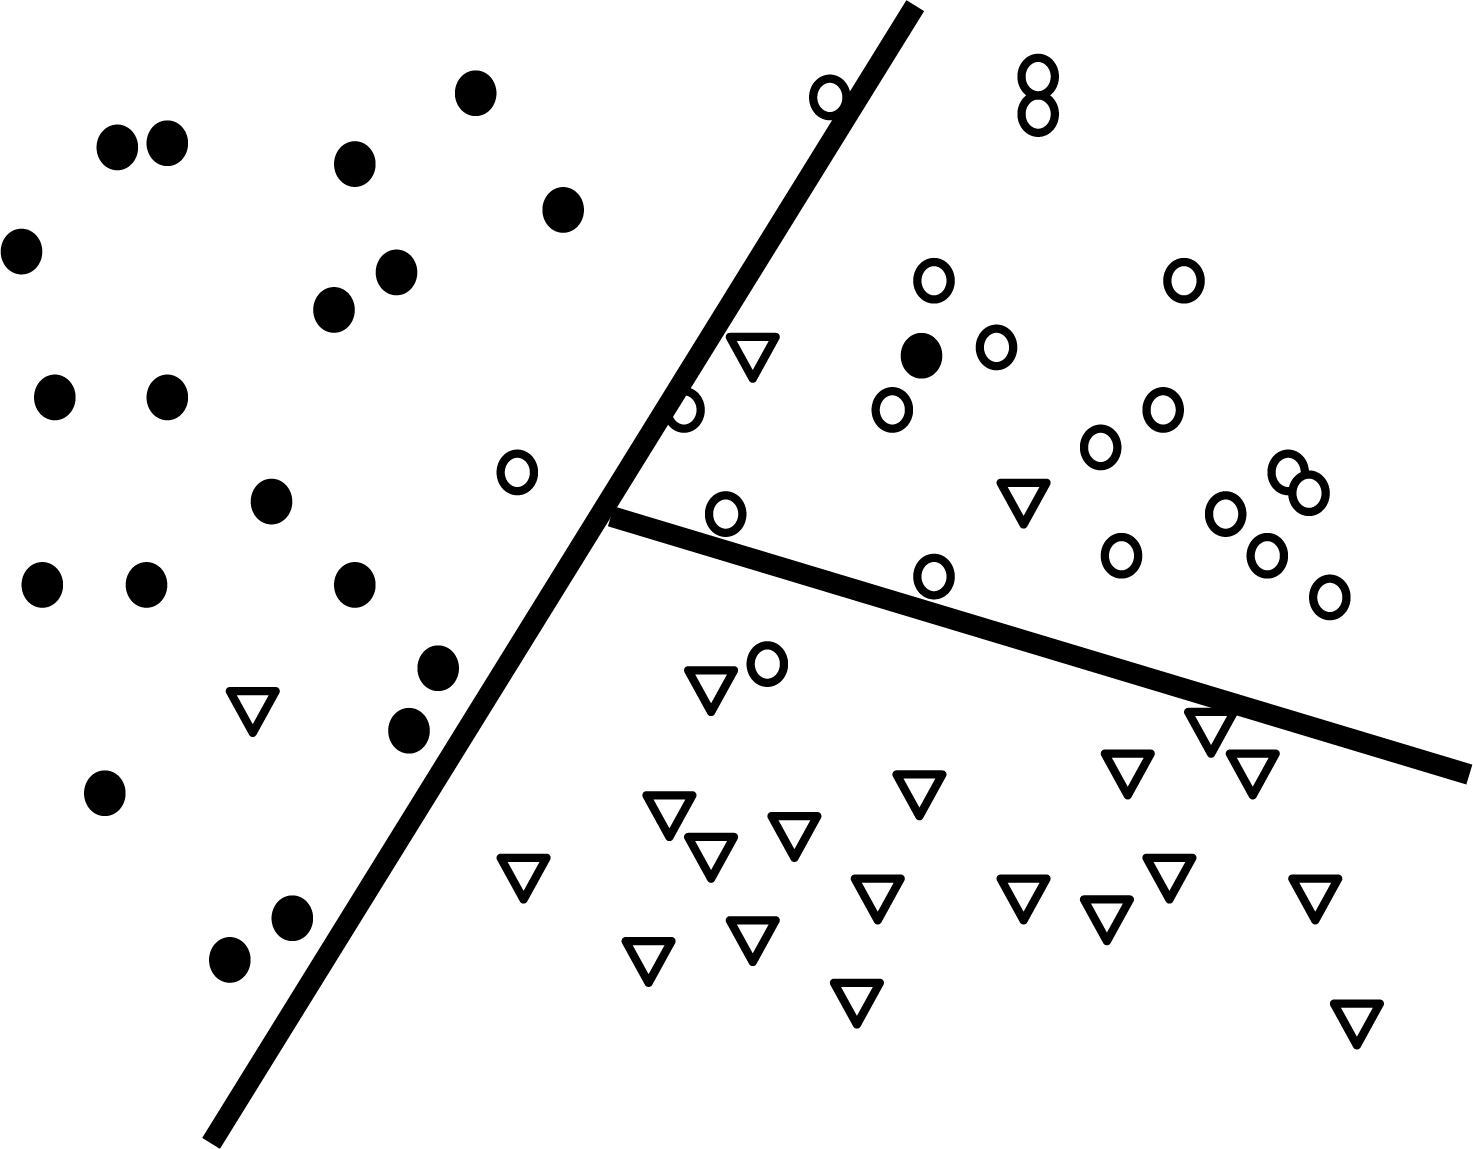
\includegraphics[width=.98\textwidth]{parts/chap-2/img-2/svm-seq.png}
            \caption{$n-1$ SVMs in a tree-based model.} 
            \label{mach:svm-model-gr-3}
        \end{subfigure}
        \caption{Comparison of different multi-class models in the feature space. In this case, there are three classes $n=3$: dots, circles and triangles.}
\end{figure}
\section{Nearest neighbour}
A classification algorithm that is often used in intrusion detection systems is the $k$-nearest neighbour ($k$-NN). This is a simple and effective method based on the distance of the elements in the feature space. Intuitively, when we want to characterize new data elements, we compare it to existent data elements and try to assign to it the characteristics --- in this case, the intrusion target --- of the similar ones. In other words, the test set elements are classified as similar training elements. Though, how do we count to elements to be similar, how do we measure similarity? In the $k$-NN algorithm, the elements are considered as data-points in the feature space and the similarity is measured as the euclidean distance between them. The most common target of the similar elements is then assigned to the test element.

More concretely, let's first consider a binary classifier of observations and targets $\left( x_1, y_1 \right), \ldots , \left( x_n, y_n \right)$ where observations $x_i \in \mathbb{R}^d$ and targets $y_i \in \left\{0,1\right\}$. To classify a new observation $\left( x_i, y_i \right)$, one just have to compare it to the $k$ other nearest observations and assign to the test observation the dominant target among its $k$ neighbours. In the classical $k$-NN algorithm, the neighbours are defined by the Euclidean distance. However, because of the monotony of the square function, one may use the square of the distances instead, avoiding to compute an extra square root, which is very useful in frameworks where operations are expensive like MPCs:
\begin{equation}
    \mathrm{d}^2\left( x_i, x_j \right) = \norm{x_i-x_j}^2 = \sum_{k=1}^d \left( x_{ik}, x_{jk} \right)^2
\end{equation}

Unlike binary classification algorithms like SVMs, $k$-NN algorithms are suited for multi-class problems without requiring any construction. However, they have also been used for binary classification in a construction \cite{Aburomman2016ASystem}. 

\subsection{Condensed Nearest Neighbours Data Reduction}
The problem of the nearest neighbours algorithm is its time to compute for large database. First, the computation of the distances increases linearly with the number of training points for each test points, thus quadratically if the number the test set has the same size as the training set. Secondly, the finding of the nearest neighbours takes requires O(kn) datapoints ... As we will see, one of the main trade-offs of MPC is the drastic increase in execution time. Therefore, the reduction of data-points becomes a necessity for the use of MPC-based $k$-NN.

The \emph{condensed nearest neighbours data reduction} (CNN) algorithm aims at finding the sole relevant data-points in the whole training set. The unclassified data-points then only need to be compared with the prototype points and not the whole database anymore. It is based on the idea that misclassified data-points lie close to the decision boundary, and one can just keep the data-points near the decision boundary and discard the others. The goal of the algorithm is to classify all training data-points into three categories:
\begin{itemize}
    \item \textbf{Outliers:} points which would not be recognized as the correct type if added to the database later. In other words, these data-points are the ones making the model perform worse with them than without. They increase the complexity of the decision boundary and increase significantly the number of kepts data-points and thus the relevance of the algorithm as it tries to keep a minimum of points defining the decision boundary. These points are to be discarded.
    \item \textbf{Prototypes:} the minimum set of points required in the training set for all the other non-outlier points to be correctly recognized. These data-points thus contain almost all of the relevant data. These points define the decision boundary and are to be kept.
    \item \textbf{Absorbed points:} points which are not outliers, and would be correctly recognized based on the sole prototype points. This could also be characterized as the redundant data. These points are far from the decision boundary and are to be discarded.
\end{itemize}

The outliers are first found by testing all existing points against the rest of the database with the chosen number $k$ of neighbours. If the point isn't recognized as the correct class, it is considered as an outlier, otherwise not. After defining all the outliers, one can proceed into the classification the restant data-points as prototypes or absorbed points. This is done in the next manner. Each point is once again tested against the dataset without the outliers, but with one sole neighbour, i.e. $k=1$. If it is well classified, it is considered as an absorbed point and can be left out of the final dataset. Otherwise, it is considered as a prototype ans is considered relevant to the classification or not redundant. These data-points are the sole ones making it to the final dataset. All points are tested until no prototype anymore makes it into the final dataset. The CNN data-reduction is given at algorithm~\ref{alg:cnn}.

In the condensed nearest neighbours algorithm, all new data-points are tested against the reduced database. Another big advantage of this algorithm is that the algorithm now always has to be used with $k=1$ because of the way we defined our prototypes and the final algorithm is thus faster. However, the classification with CNN will most of the time lead to a slightly different classification than with the classical $k$-NN against the whole dataset. Let's now investigate the classification trade-off in the case of our intrusion detection system database. 

\begin{center}
\begin{algorithm}[H]
 \KwData{Set $\mathcal{S}$ of $n$ feature points $\left\{x_i\right\}_{i=1 \ldots n}$ and corresponding targets $\left\{y_i\right\}_{i=1 \ldots n}$, number of neighbours $k$ for outlier detection}
 \KwResult{Reduced set $\mathcal{R}$ of $m<n$ feature points $\left\{x_i\right\}_{i=1 \ldots m}$ and corresponding targets $\left\{y_i\right\}_{i=1 \ldots m}$}
\DontPrintSemicolon
\SetKwFunction{FkNN}{kNN}

\ForEach{$\left(x_i, y_i\right) \in \mathcal{S}$}{
$t \leftarrow $\FkNN{$k$, $x_i$, $\mathcal{S}$} \;
\lIf{$t \neq y_i$}{remove chosen $\left(x_i, y_i\right)$ from $\mathcal{S}$}
}
$\mathcal{R}_0 \leftarrow \emptyset$ \;
add random $\left(x_i, y_i\right)$ to $\mathcal{S}$ \;

\Repeat{$\mathcal{R}_0 = \mathcal{R}_1$}{
$\mathcal{R}_1 \leftarrow \mathcal{R}_0$ \;
\For{$\left(x_i, y_i\right) \in \mathcal{S}$}{
$s \leftarrow $\FkNN{$k=1$, $x_i$, $\mathcal{R}_1$} \;
\lIf{$s \neq y_i$}{add $\left(x_i, y_i\right)$ to $\mathcal{R}_1$}
}
}
\Return{$\mathcal{R}_1$}
\caption{The condensed nearest neighbours algorithm. This algorithm relies on an implementation of the $k$-NN, represented here by the $\mathtt{kNN}$ function that takes as input the number of neighbours $k$, the data-points to be classified $x_i$ and the set in which it should search for the neighbours $\mathcal{S}$.}
\label{alg:cnn}
\end{algorithm}
\end{center}
\section{Ensemble methods}
\subsection{Bagging}
Bagging, short for \emph{boostrap aggregating} has first been described by Breiman \cite{Breiman1996BaggingPredictors}. Instead of one instance of a model trained on a whole learning set, different instances are trained with different bootstrap replicates of the original learning set. The final inference is then made by a majority vote on the different results. In other words, this method averages the set of the different possible learned models and reduces the instability of the prediction method. 

Let's consider a data-set of $N$ elements $\mathcal{L}=\left\{ \left( x_n,y_n\right),n=1,...,N\right\}$ where $x$ is the input vector and $y$ the output vector. The idea is to minimise the variation of the predictor $\hat{y}=\phi\left(x,\mathcal{L}\right)$ by calculating its expectation over the distribution of $\mathcal{L}$
\begin{equation}
    \phi_A\left(x,\mathcal{L}\right) = \mathbb{E}_\mathcal{L} \phi\left(x,\mathcal{L}\right) \approx A \left( \left\{ \phi\left(x,\mathcal{L}_k\right) \right\} \right) \qquad k=1,\, \ldots,\, N_k
\end{equation}
where $A$ is an aggregation function (\emph{i.e.} mean for a regression or a majority vote for a classification) and $\mathcal{L}_k$ different instances of the distribution of $\mathcal{L}$. As the instances set $\{ \mathcal{L}_k \}$ is not available, a bootstrap set $\{\mathcal{L}^{(B)}\}$ is constructed, each instance consisting of $N$ elements drawn randomly from the original $\mathcal{L}$, but \emph{with replacement}. The average prediction is then calculated as
\begin{equation}
    \phi_B\left(x,\mathcal{L}\right) = A(\{ \phi(x,\mathcal{L}^{(B)}) \})
\end{equation}
In his experiments, Breiman noted that 25 a 50 bootstrap replicates $N_k$ seemed a reasonable choice. In a certain sense, one could see bagging as a variant of cross-validation method on the whole learning process: a sort of \emph{cross-learning} with replacement.

The reason why bagging works is the much lower mean-squared prediction error of $\phi_A$ compared to $\phi$. Nevertheless, the fact of using the available $\phi_B$ instead of the theoretical $\phi_A$ has also drawbacks as it can deteriorate the prediction of already stable classifiers. In other words, bagging unstable classifiers such as neural nets, classification and linear regressions, usually improves them, whereas bagging usually stable classifiers such as $k$-nearest neighbours is not a good idea \cite{Breiman1996HeuristicsSelection}.

\subsection{Influence of MPC}
Compare naïve bootstrapping (each bootstraps its own copy) and full bootstrapping as described above. Can be done in parallel (MPC wins a lot from parallelization).

\subsubsection{Boosting}
The boosting method is based on a proof by Schapire \cite{Schapire1989} that weak learnability, an algorithm that slightly out-performs a random classifier, is equivalent to a strong classifier. To prove this equivalence, he used an algorithm that sequentially trains classifiers. Each classifier has a training set consisting of half well-classified elements of the previous one and half of wrongly classified elements, the first classifier starting from the original training set. Based on this idea, a later algorithm, called \emph{adaptive boosting} was developed based on a better distribution of the missclassified elements for creating the subsequent training sets \cite{Freund1997ABoosting}. + majority vote from all classifiers.

+ intuitively the algorithm will perform better when learning from the more difficult elements. In a certain sense, the more complex elements will have more degrees of freedom (not sure of this one).
\section{Models tested}



\FloatBarrier

\FloatBarrier